\documentclass[border=10pt]{standalone}
\usepackage[svgnames]{xcolor}
\usepackage{amsmath}
\usepackage{pgfplots}
\pgfplotsset{compat=newest}
\usepackage[sfdefault]{FiraSans}
\usepackage{FiraMono}
\renewcommand*\familydefault{\sfdefault}
\begin{document}
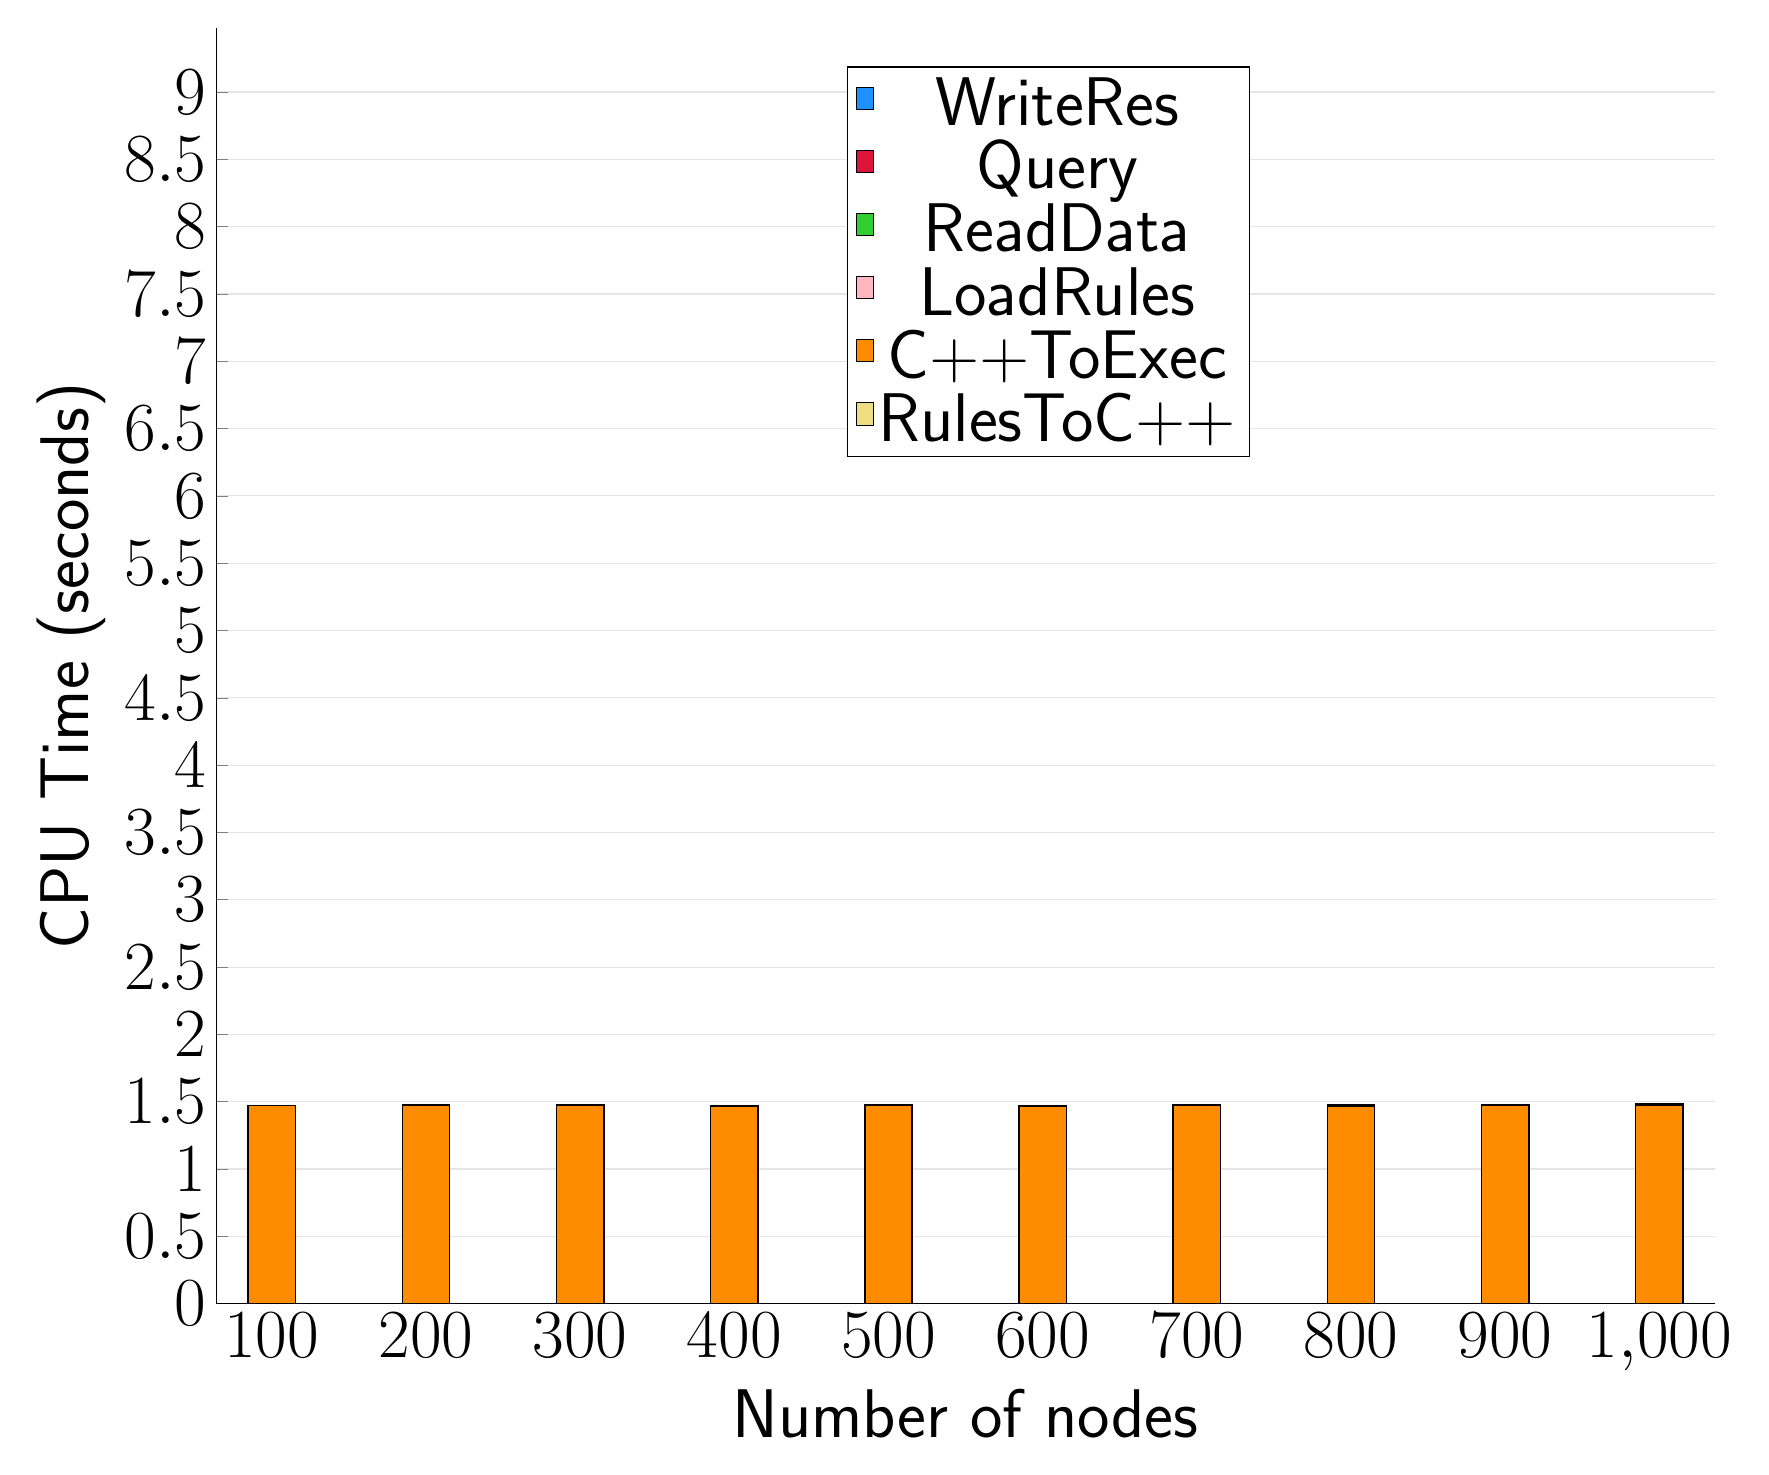
\begin{tikzpicture}
\begin{axis}[
   ybar stacked,
   width=1.7\textwidth,
   bar width=0.6cm,
   ymajorgrids, tick align=inside,
   major grid style={draw=gray!20},
   xtick=data,
   ymin=0, ymax=9.474,
   axis x line*=bottom,
   axis y line*=left,
   enlarge x limits=0.04,
   legend style={
       at={(0.69, 0.97)},
       anchor=north east,
       legend columns=1,
       font=\Huge,
   },
   ylabel={CPU Time (seconds)},
   xlabel={Number of nodes},
   label style={font=\Huge},
   tick label style={font=\Huge},
]
\addlegendimage{fill=DodgerBlue, draw=black, line width=0.2pt}
\addlegendentry{WriteRes}
\addlegendimage{fill=Crimson, draw=black, line width=0.2pt}
\addlegendentry{Query}
\addlegendimage{fill=LimeGreen, draw=black, line width=0.2pt}
\addlegendentry{ReadData}
\addlegendimage{fill=LightPink, draw=black, line width=0.2pt}
\addlegendentry{LoadRules}
\addlegendimage{fill=DarkOrange, draw=black, line width=0.2pt}
\addlegendentry{C++ToExec}
\addlegendimage{fill=LightGoldenrod, draw=black, line width=0.2pt}
\addlegendentry{RulesToC++}
\addplot +[fill=LightGoldenrod, draw=black, line width=0.55pt] coordinates {
(100, 0.0020000000000000005)
(200, 0.0)
(300, 0.0)
(400, 0.0)
(500, 0.0)
(600, 0.0)
(700, 0.0)
(800, 0.0)
(900, 0.0)
(1000, 0.0020000000000000005)
};
\addplot +[fill=DarkOrange, draw=black, line width=0.55pt] coordinates {
(100, 1.47)
(200, 1.472)
(300, 1.472)
(400, 1.468)
(500, 1.472)
(600, 1.4659999999999997)
(700, 1.474)
(800, 1.468)
(900, 1.472)
(1000, 1.472)
};
\addplot +[fill=LightPink, draw=black, line width=0.55pt] coordinates {
(100, 0.0001536)
(200, 0.00018740000000000003)
(300, 0.000193)
(400, 0.0001992)
(500, 0.0001876)
(600, 0.0001906)
(700, 0.00019559999999999998)
(800, 0.0001964)
(900, 0.0001806)
(1000, 0.0001858)
};
\addplot +[fill=LimeGreen, draw=black, line width=0.55pt] coordinates {
(100, 0.000658)
(200, 0.0011676)
(300, 0.0014114000000000002)
(400, 0.0019241999999999998)
(500, 0.0023072)
(600, 0.0025944)
(700, 0.0030258)
(800, 0.0034043999999999997)
(900, 0.0035558)
(1000, 0.0038378)
};
\addplot +[fill=Crimson, draw=black, line width=0.55pt] coordinates {
(100, 0.00023140000000000001)
(200, 0.0005484)
(300, 0.000683)
(400, 0.0010072)
(500, 0.0012798)
(600, 0.0015002000000000001)
(700, 0.0017372)
(800, 0.0019682)
(900, 0.0021226)
(1000, 0.002633)
};
\addplot +[fill=DodgerBlue, draw=black, line width=0.55pt] coordinates {
(100, 0.000333)
(200, 0.0006118)
(300, 0.0005855999999999999)
(400, 0.0007854)
(500, 0.0008432)
(600, 0.0007878)
(700, 0.0009362000000000001)
(800, 0.0009850000000000002)
(900, 0.0009544)
(1000, 0.0009784)
};
\end{axis}
\end{tikzpicture}

\end{document}
